\section{Case Analysis and Visualization}

\subsection{Spectral templates of four representative words}

Figure~\ref{fig:matlab-spectra} shows the short-time FFT templates of four representative words in the MATLAB demonstration. The figure is not a training summary. Its purpose is to show the actual shape of the local templates.

\begin{figure}[H]
    \centering
    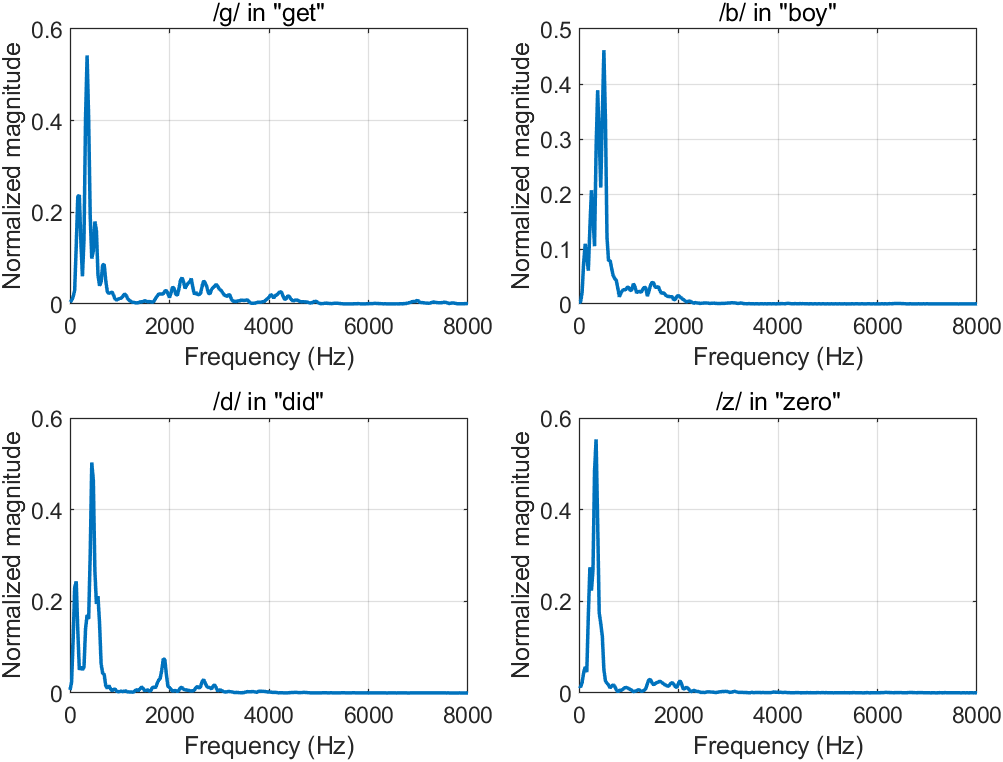
\includegraphics[width=0.95\textwidth]{figures/course_matlab/example_short_time_spectra.png}
    \caption{Short-time FFT magnitude templates of four representative words.}
    \label{fig:matlab-spectra}
\end{figure}

The figure shows a clear contrast. The high-frequency frication of /z/ lasts longer, the initial releases of /b/ and /d/ are shorter, and the short-time structure of /g/ is the easiest to blur when alignment shifts in time. This pattern is consistent with the class templates constructed by our method.

\subsection{Correlation score matrix}

Figure~\ref{fig:matlab-score} gives the correlation score matrix produced by the same set of templates on the four representative words. The figure is not meant to prove that the model is strong. It shows that the basic operation of template-query correlation is actually working.

\begin{figure}[H]
    \centering
    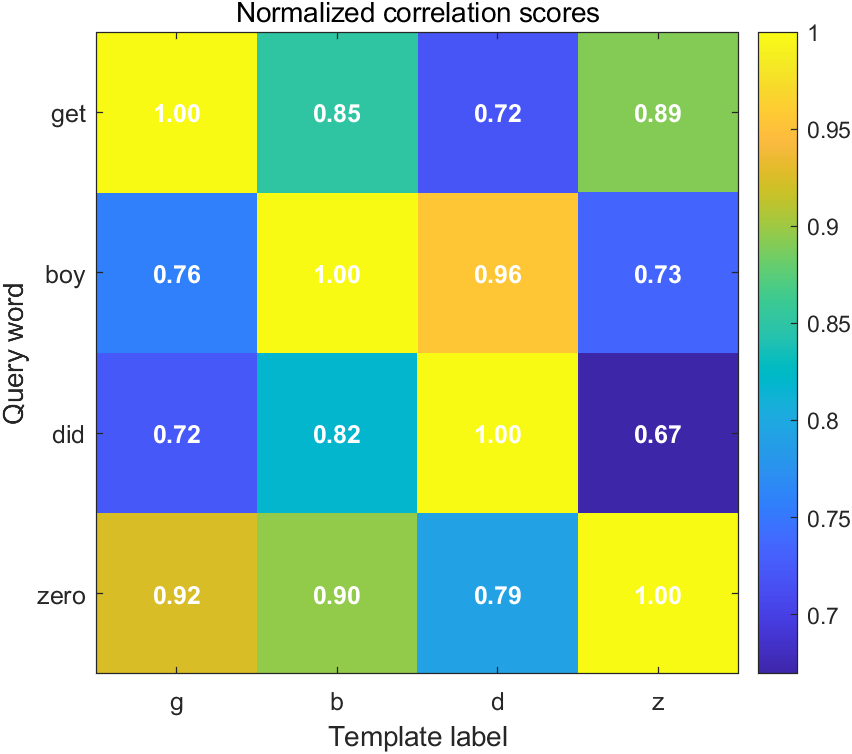
\includegraphics[width=0.70\textwidth]{figures/course_matlab/example_score_matrix.png}
    \caption{Correlation score matrix for four representative words.}
    \label{fig:matlab-score}
\end{figure}

This matrix is more direct than the waveform alone because it turns the question of which template looks most similar to a local speech segment into a numerical comparison. When the score gap is small, the alignment of the initial consonant is usually not stable enough. This is also the problem that the later AI reimplementation tries to address.
